\documentclass[4paper,10pt]{paper}

\usepackage{xeCJK}
\usepackage{amsmath}
\setCJKmainfont{AR PL UKai CN}

\title{Homework 2}
\author{昂伟 PB11011058}
\date{ \today }

\begin{document}

\maketitle

\section*{problem 1}

\begin{align*}
			&(\lambda p.\lambda q.\lambda r.p\ q\ r)(\lambda p.\lambda q.p\ q\ r)\\
\rightarrow & (\lambda s.\lambda t.\lambda u.s\ t\ u)(\lambda p.\lambda q.p\ q\ r)\\
\rightarrow & \lambda t.\lambda u.(\lambda p.\lambda q.p\ q\ r)t\ u \\
\rightarrow & \lambda t.\lambda u.(\lambda q.t\ q\ r)u \\
\rightarrow & \lambda t.\lambda u.t\ u\ r \\
\rightarrow & r
\end{align*}

\par \textit{If we don't rename bound variables, free variable $r$ be bound. So
rename bound variables so that all bound variables are different from
each other and different from all of the free variables.}

\section*{problem 5}

(a)$$<x+y,\sigma> \: \rightarrow \: <2+y,\sigma> \: \rightarrow \: <2+3,\sigma> \: \rightarrow<5,\sigma>$$

(b)$$<x=x+3,\sigma> \: \rightarrow \: <x=1+3,\sigma> \: \rightarrow<x=4,\sigma> \: \rightarrow \: <4,Put(\sigma,x,4)>$$

(c)$$<(x=3)+x,\sigma> \:\rightarrow \: <3+x,Put(\sigma,x,3)> \: \rightarrow \: <3+3,\sigma'> \: \rightarrow \: <6,\sigma'>$$

 (d)
 	\begin{align*}
 				 & <x=(x=x+3)+(x=x+5),\sigma> \\
 	 \rightarrow & <x=(x=1+3)+(x=x+5),\sigma>\\
	 \rightarrow & <x=(x=4)+(x=x+5)\sigma> \\
	 \rightarrow & <x=4+(x=x+5),Put(\sigma,x,4)>\\
	 \rightarrow & <x=4+(x=4+5),\sigma'> \\
	 \rightarrow & <x=4+(x=9),\sigma'>\\
	 \rightarrow & <x=4+9,Put(\sigma',x,9)> \\ 
	 \rightarrow &<x=13,\sigma''> \\
	 \rightarrow & <13,Put(\sigma'',x,13)>
	\end{align*}
	

\section*{problem 6}
(a) 2 (b) 4 (c) 3

\section*{problem 7}

(a) $\omega=8$

(b)
\begin{center}
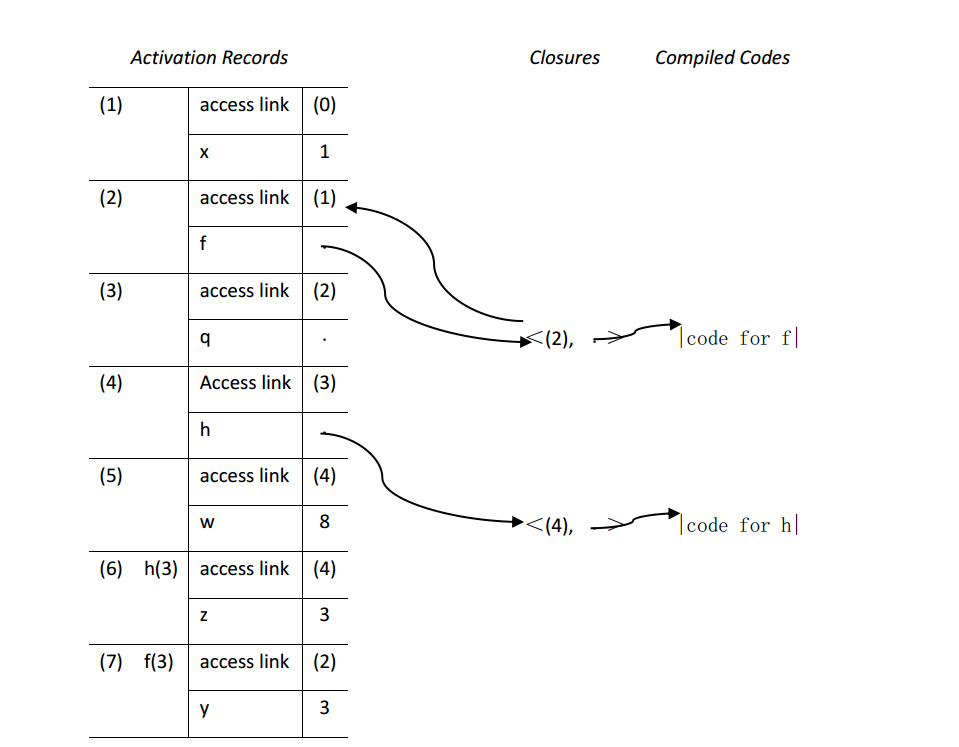
\includegraphics[scale=0.48]{7.png}
\end{center}

\pagebreak
\section*{problem 8}
(a)
\begin{center}
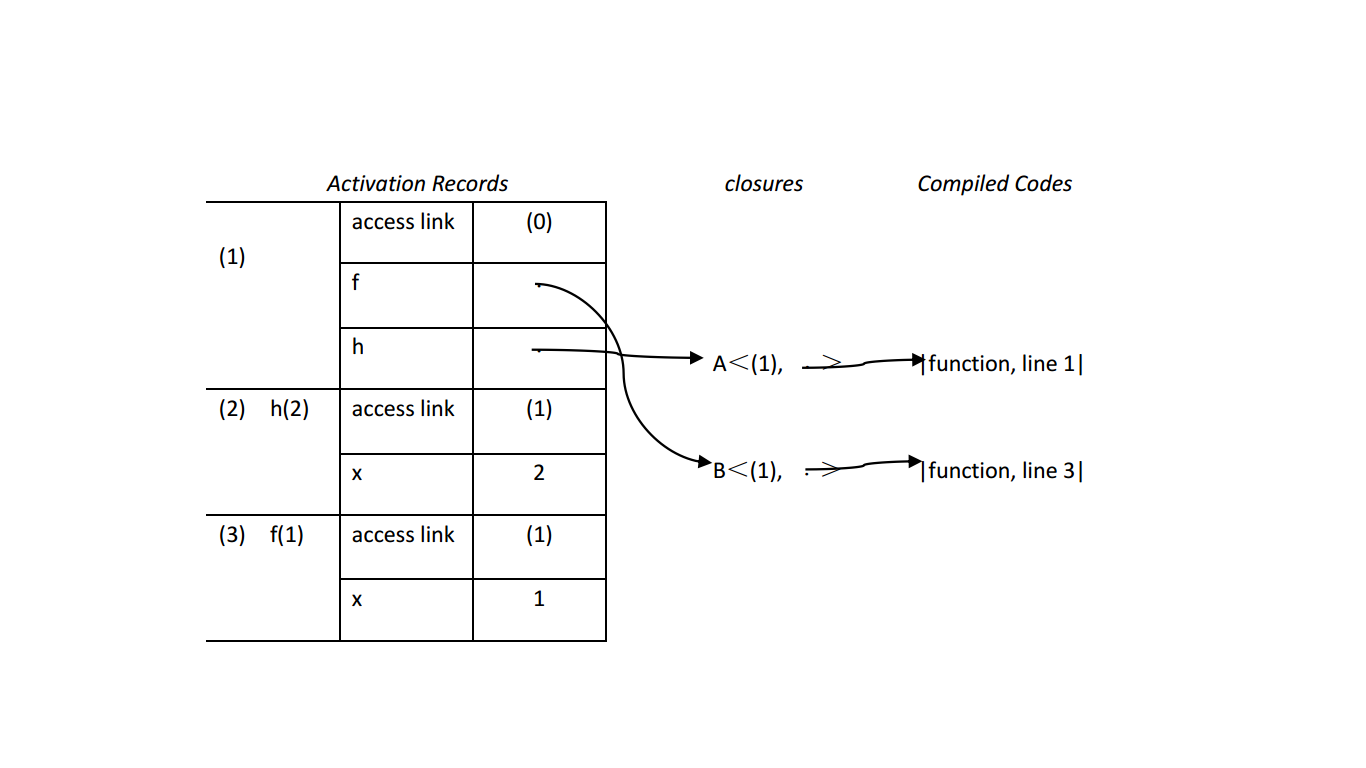
\includegraphics[width=1.2\textwidth]{8(a).png}
\end{center}

(b) B

(c) When calling function $h(2)$ after line 2, first function $f_{1}(2)$ will be called, then function $f_{1}(1)$; When calling function $h(2)$ on line 4,function $f_{1}(2)$ will be called firstly,then $f_{3}(1)$ will be called because on line 3 $f$ is modified be point to function $f_{3}$.

\pagebreak
(d)\\
\begin{center}
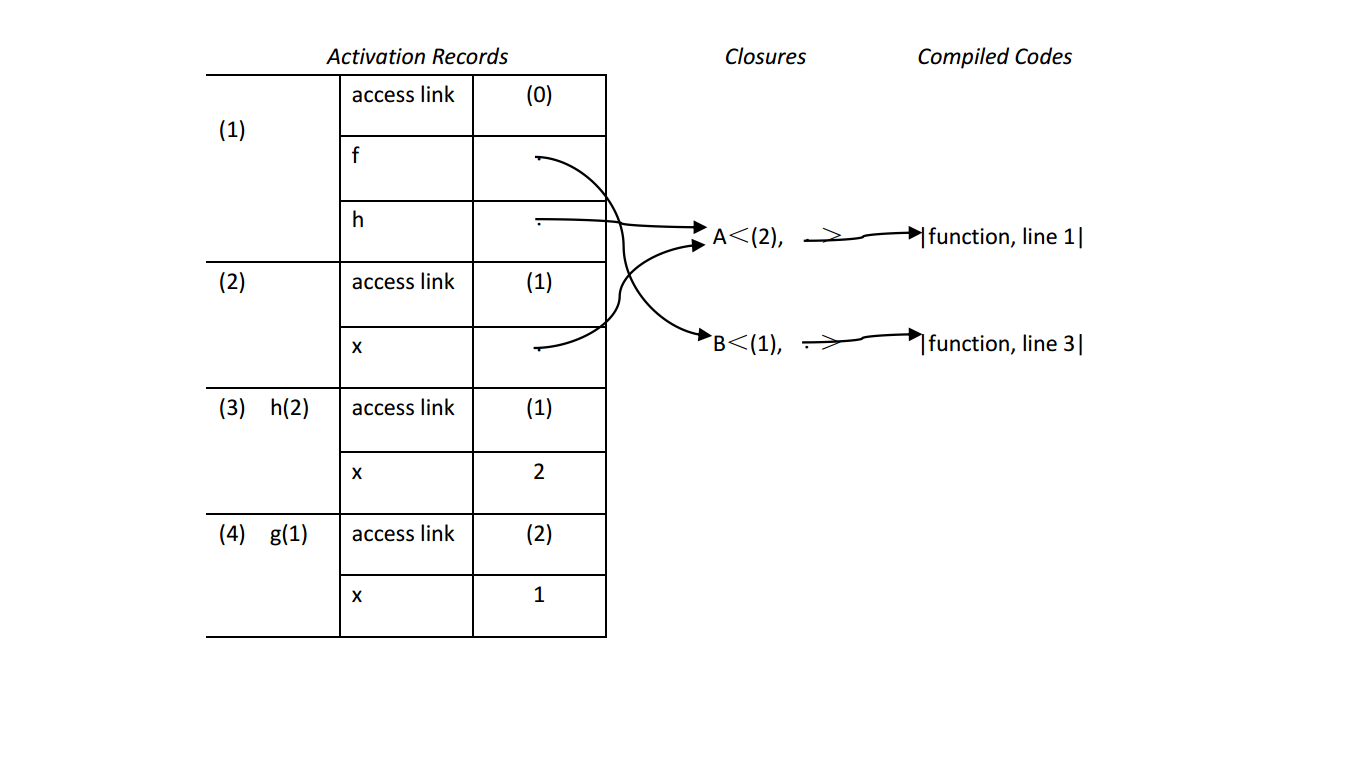
\includegraphics[width=1.2\textwidth]{8(d).png}
\end{center}

(e)$h(2)=2$. $g(2)$ is called firstly, then $g(1)$.

\end{document}
